\extrafloats{100}
\chapter{Methods}

\section{JESRON MARUDUT HATUAN/1164077}
\subsection{Teori}
Penyelesaian Tugas Harian 5
\begin{enumerate}
\item Random Forest dan Ilustrasi Gambar
\begin{itemize}
\item Pengertian Random Forest:

Random forests merupakan sebuah metode dalam pembelajaran untuk klasifikasi, regresi dan tugas-tugas lain yang telah berperasi dengan membangun banyak pohon keputusan pada saat latihan hingga menciptakan kelas yang merupakan mode kelas atau klasifikasi atau beberapa prediksi dari setiap tree atau pohon.

\item Ilustrasi Gambar Random Forest :
\begin{figure}[ht]
\centering
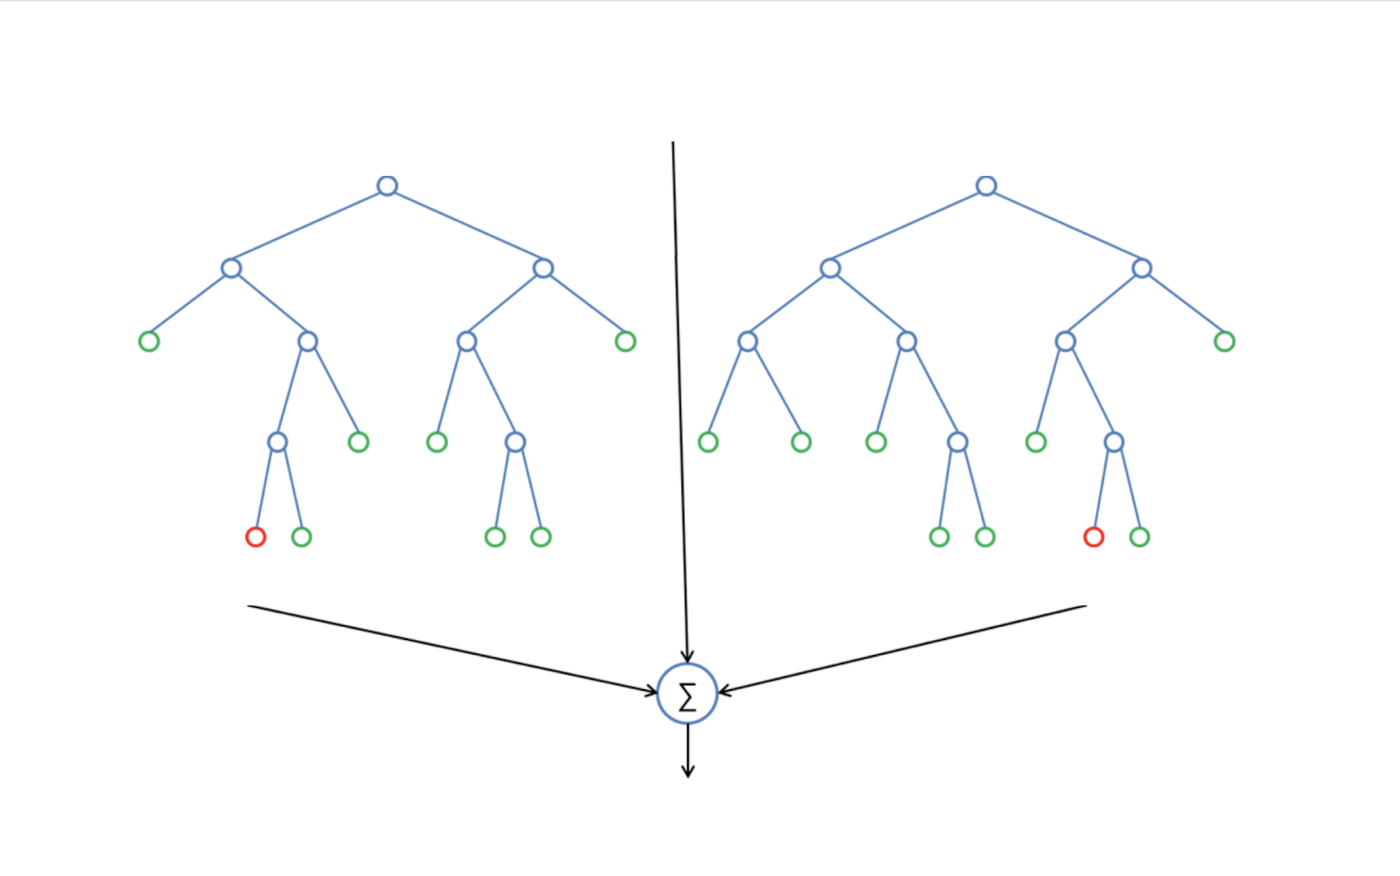
\includegraphics[scale=0.5]{figures/c3jesron1.png}
\caption{Gambar Random Forest}
\label{contoh}
\end{figure}
\end{itemize}
\item Langkah-langkah Membaca Dataset

Berikut adalah langkah-langkah membaca dataset :
\begin{itemize}
\item Pertama-tamma buka applikasi Anaconda Navigator lalu jalankan Syder, kemudian import libraries yang mau dibuat
\item Selanjutnya masukkan kode python untuk membaca file csv, lalu run applikasinya
\begin{figure}[ht]
\centering
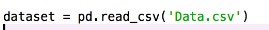
\includegraphics[scale=0.8]{figures/c3jesron2.jpeg}
\caption{Gambar Code Python}
\label{contoh}
\end{figure}

\item Maka pada jendela konsol akan menampilkan pesan berikut:

\begin{figure}[ht]
\centering
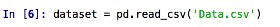
\includegraphics[scale=0.8]{figures/c3jesron3.jpeg}
\caption{Gambar Output}
\label{contoh}
\end{figure}

\item Dan dari jendela explorer akan tampil dataset yang sudah diimport.

\begin{figure}[ht]
\centering
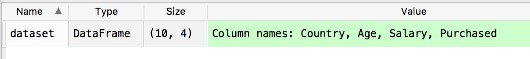
\includegraphics[scale=0.5]{figures/c3jesron4.jpeg}
\caption{Gambar Import Dataset}
\label{contoh}
\end{figure}

\item Selanjutnya klik dataset cell, maka akan muncul seperti berikut :
\item Seperti yang terlihat pada gambar tersebut dataset ini memiliki Kolom Country, Age, dan Salary sebagai kolom

\begin{figure}[ht]
\centering
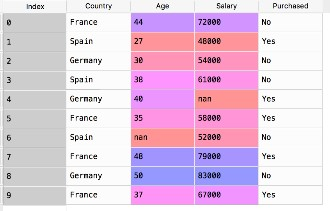
\includegraphics[scale=0.5]{figures/c3jesron5.jpeg}
\caption{Gambar Hasil Dataset Sel}
\label{contoh}
\end{figure}

\item Purchased sebagai dependent variable-nya.
\item Selanjutnya buat 2 matrix of features yang berisi values dari independent variable dan dependent variable.
\item Selanjutnya, masukan perintah berikut :

\begin{figure}[ht]
\centering
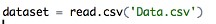
\includegraphics[scale=0.8]{figures/c3jesron6.jpeg}
\caption{Gambar Masukkan Perintah}
\label{contoh}
\end{figure}

\item Perintah yang telah dilakukan gunanya untuk menampilkan dataset.
\item Lalu klick dataset tersebut maka muncul tabel berisi dataset.
\end{itemize}
\item Cross Validation

Cross Validation adalah sebuah teknik untuk memvalidasi model agar dapat menilai bagaimana hasil dari sebuah statistik analisis yang akan menggeneralisasi kumpulan beberapa data independen. Teknik ini lebih sering digunakan untuk melakukan prediksi model dan memperkirakan seberapa akurat sebuah model prediktif ketika sedang dijalankan dalam sebuah praktiknya. Dalam sebuah masalah prediksi, sebuah model biasanya diberikan kumpulan data (dataset) yang telah diketahui untuk digunakan dalam menjalankan pelatihan (dataset pelatihan), serta kumpulan data yang tidak diketahui (atau data yang pertama kali dilihat) terhadap model yang diuji (pengujian dataset)

\item Maksud dari score 44\% pada random forest, 27\% pada decission tree dan 29\%dari SVM.

Maksud dari score 27\% pada decission tree adalah hasil dari  presentasi dari perhitungan dataset, sedangkan maksud dari score 29\% pada SVM adalah dengan pendekatan jaringan saraf. Hasilnya didapat dari valdasi silang untuk memastikan bahwa membagi training test dengan cara yang berbeda. Sehingga outputnya 44\% untuk hutan acak, 27\% untuk pohon keputusan, dan 29\% untuk SVM.

\item Confusion Matrix Dan Ilustrasinya
\begin{enumerate}
\item Perhitungan confusion matrix adalah sebagai berikut, akan saya beri contoh sederhana yaitu pengambilan keputusan untuk mendapatkan bantuan beasiswa. Saya menggunakan dua atribut, yaitu rekening listrik dan gaji. Ini adalah pohon keputusannya:
\begin{figure}[ht]
\centering
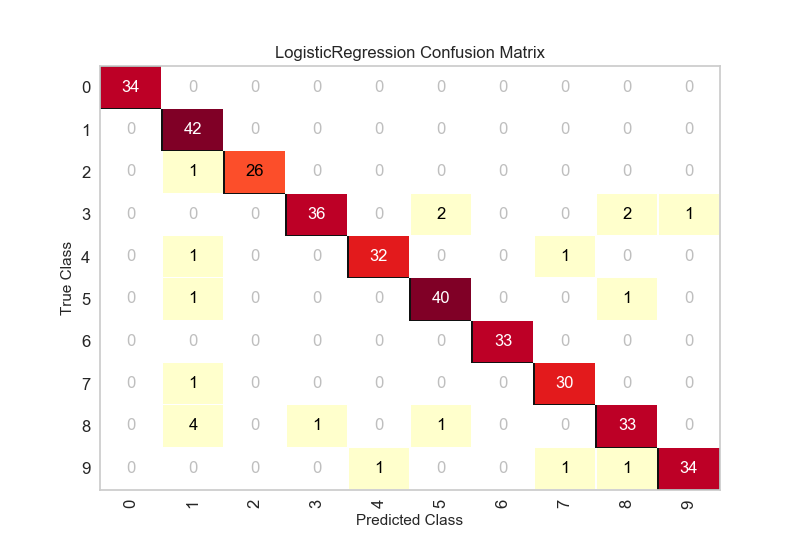
\includegraphics[scale=0.5]{figures/c3jesron7.png}
\caption{Pohon Keputusan}
\label{contoh}
\end{figure}
\end{enumerate}

Selanjutnya data testingnya adalah

\begin{figure}[ht]
\centering
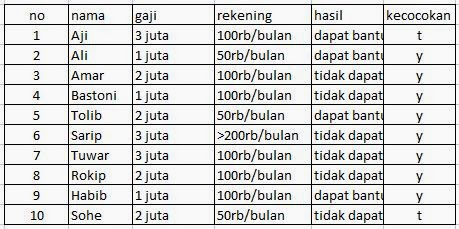
\includegraphics[scale=0.5]{figures/c3jesron8.jpg}
\caption{Gambar Data Testing}
\label{contoh}
\end{figure}

Pertama-pertama, kita lakukan adalah mencari 4 nilai yaitu a,b,c, dan d:

a= 5

b= 1

c= 1

d= 3

Hingga kita dapat mencari nilai Recall, Precision, accuracy dan Error Rate

Recall =3/(1+3) = 0,75

Precision = 3/(1+3) = 0,75

Accuracy =(5+3)/(5+1+1+3) = 0,8

Error Rate =(1+1)/(5+1+1+3) = 0,2

\item Voting Random Forest Dan Ilustrasi Gambarnya.

\begin{itemize}
\item Pengertian Voting pada Random Forest
Voting yaitu suara untuk setiap target yang diprediksi pada saat melakukan Random Forest. Pertimbangkan target prediksi dengan voting tertinggi sebagai prediksi akhir dari algoritma random forest.

\item Gambar Voting Random Forest :
\begin{figure}[ht]
\centering
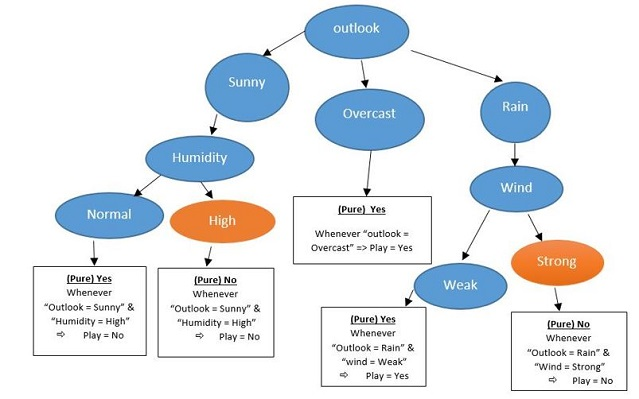
\includegraphics[scale=0.8]{figures/c3jesron9.jpg}
\caption{Gambar Voting Random Forest}
\label{contoh}
\end{figure}
\end{itemize}
\end{enumerate}
\section{The data}
PLease tell where is the data come from, a little brief of company can be put here.
\section {Puad Hamdani/ 1164084}
\subsection {Teori}
\begin{enumerate}
\item Random Forest
\par
Merupakan classifier yang terdiri dari banyak pohon keputusan dan melakukan klasifikasi berdasarkan keluaran dari hasil klasifikasi setiap pohon keputusan anggota
\begin{figure}[ht]
\centering
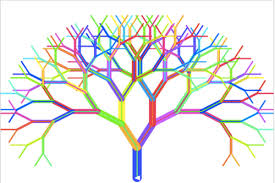
\includegraphics[scale=0.5]{figures/111.JPG}
\caption{Random Forest}
\end{figure}
\item Cara membaca dataset kasus
\begin{itemize}
\item Buka aplikasi spyder untuk membuka dan membaca kodingan dataset
\item Kemudian buat  variable imgatt untuk memasukkan atribut label
\item Lalu uji coba kodingan untuk mengetahui apa hasil dari dataset tersebut
\item imgatt.head() untuk melihat sebagian data awal
\item .shape untuk melihat jumlah data
\item .pivot untuk merubah atribut menjadi kolom
\par
Dengan menguji coba kodingan yang ada pada spyder untuk membaca data set.
\end{itemize}
\item Cross Validation
\par 
Cross Validation adalah teknik validasi model untuk menilai bagaimana hasil analisis statistik (model) akan digeneralisasi ke kumpulan data independen. terutama digunakan dalam pengaturan di mana tujuannya adalah prediksi, dan orang ingin memperkirakan seberapa akurat model prediksi akan dilakukan dalam praktek
\item Arti 44 persen pada RF, 27 persen pada Decission Tree, dan 29 persen pada SVM.
\begin{itemize}
\item Merupakan akurasi dari sebuah pohon keputusan untuk menunjukkan hasil keputusan dengan klasifikasi dari dataset yang ada.
\end{itemize}
\item Confusion Matrix
\begin{itemize}
\item Import confusion matrix
\item Plot confusion matrix
\item Lalu sesuaikan plotnya
\item Setelah itu plot kembali
\end{itemize}
\item Voting
\par
Voting Merupakan metode untuk menentukan keputusan dalam suatu suatu pemilihan, berdasarkan pendapat per orang, dan keputusan ditentukan berdasarkan pemilih terbanyak
\end{enumerate}

\section {Jesron Marudut Hatuan / 1164077}
\subsection{Praktek}
Tugas Harian ke-2
\begin{enumerate}
\item Aplikasi Sederhana Pandas dan Penjelasan Code ( Perbaris )
\begin{itemize}
\item Pandas:
\par 
\par
\begin{itemize}
\item Baris1 :  Mengimport library pandas dari python dengan inisiasi pd.
\par
\item Baris 2 : Parameter data ini diisi dengan data yang akan dibuat seriess.
\par
\item Baris 3 : Mengubah data karakter menjadi series
\par
\item Baris 4 : Mempilkan karakter
\par
\end{itemize}
\item Hasil:
\par
\par
\begin{figure}[ht]
\centering
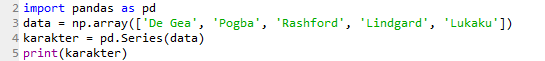
\includegraphics[scale=0.8]{figures/hmm/1.png}
\caption{Applikasi sederhana Pandas}
\label{contoh}
\end{figure}
\par

\par
\par
\item Aplikasi Sederhana Numpy dan Penjelasan Code ( Perbaris )
\begin{itemize}
\item Code Numpy:
\par 
\par
\begin{itemize}
\item Baris 1 : Mengimport library numpy dari python dengan inisiasi np
\par
\item Baris 2 : Parameter data ini diisi dengan data yang akan dibuat seriess.
\par
\item Baris 3 : Mengubah data karakter menjadi series
\par
\item Baris 4 : Mempilkan karakter
\par
\end{itemize}
\item Hasil:
\par
\par
\begin{figure}[ht]
\centering
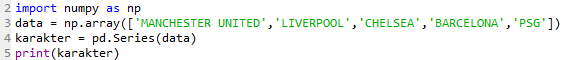
\includegraphics[scale=0.8]{figures/hmm/2.png}
\caption{Applikasi Numpy}
\label{contoh}
\end{figure}
\par
\par

\par
\par
\item Aplikasi Sederhana Matplotlib dan Penjelasan Code ( Perbaris )
\begin{itemize}
\item Code Matplotlib:
\par 
\par
\begin{itemize}
\item Baris 1 : Mengimport library matplotlib dari python dengan inisiasi jes.
\par
\item Baris 2 : Menampilkan variabel dari x dan variabel y
\par
\item Baris 3 : Menampilkan inisiasi jes dari variable X dan Y
\par
\end{itemize}
\item Hasil:
\par
\par
\begin{figure}[ht]
\centering
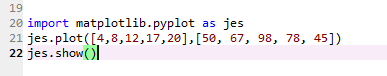
\includegraphics[scale=0.8]{figures/hmm/3.png}
\caption{Applikasi Matplotlib}
\label{contoh}
\end{figure}
\par
\end{itemize}

\par
\par
\item Program Aplikasi Random Forest dan Penjelasan Keluarannya :
\begin{itemize}
\item Kode Random Forest 1 :
\par
\begin{figure}[ht]
\centering
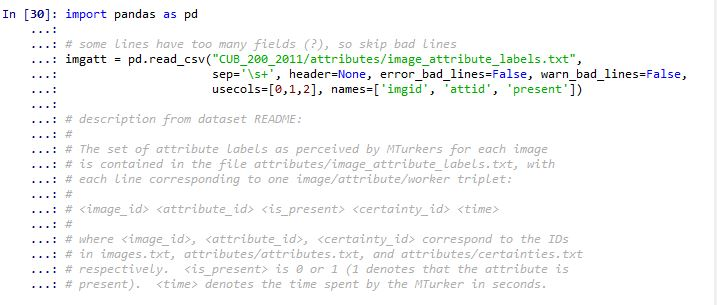
\includegraphics[scale=0.7]{figures/hmm/cod1.jpg}
\caption{Gambar ke-1}
\label{contoh}
\end{figure}
\par
\begin{itemize}
\item Penjelasan : Untuk membaca dataset. Kodingan tersebut menghasilkan variabel baru yaitu imgatt dan terdapat 3 kolom dan 3677856 baris data.
\par 
\par
\end{itemize}
\item Kode Random Forest 2 :
\par
\begin{figure}[ht]
\centering
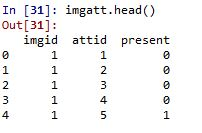
\includegraphics[scale=0.7]{figures/hmm/cod2.jpg}
\caption{Gambar ke-2}
\label{contoh}
\end{figure}
\par
\begin{itemize}
\item Penjelasan : Kodingan berikut berfungsi untuk melihat sebagian data awal dari dataset. Dan hasilnya akan terdapat pada gambar di atas setelah di eksekusi.
\par
\par
\end{itemize}
\item Kode Random Forest 3 :
\par
\begin{figure}[ht]
\centering
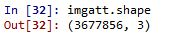
\includegraphics[scale=0.7]{figures/hmm/cod3.jpg}
\caption{Gambar ke-3}
\label{contoh}
\end{figure}
\par
\begin{itemize}
\item Penjelasan : Kodingan diatas merupakan gambaran untuk menampilkan hasil dari dataset yang telah di eksekusi. Dimana pada gambar di atas 3677856 merupakan baris dan 3 adalah kolom.
\par
\par
\end{itemize}
\item Kode Random Forest 4 :
\par
\begin{figure}[ht]
\centering
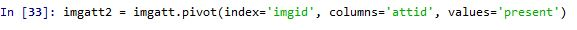
\includegraphics[scale=0.7]{figures/hmm/cod4.jpg}
\caption{Gambar ke-4}
\label{contoh}
\end{figure}
\par
\begin{itemize}
\item Penjelasan : Gambar di atas menampilkan hasil dari variabel imgatt2. Dimana index nya 'imgid', kolom berisi 'attid' dan values atau nilainya berisi 'present'.
\par
\par
\end{itemize}
\item Kode Random Forest 5 :
\par
\begin{figure}[ht]
\centering
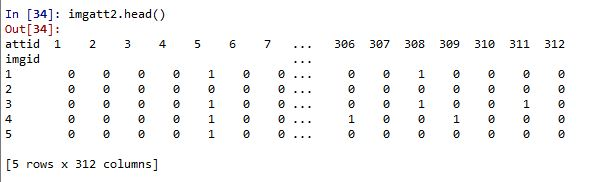
\includegraphics[scale=0.7]{figures/hmm/cod5.jpg}
\caption{Gambar ke-5}
\label{contoh}
\end{figure}
\par
\begin{itemize}
\item Penjelasan :Gambar diatas menampilkan hasil dari variabel imgatt2.head, dimana dataset nya ada 5 baris dan 312 kolom.
\par
\par
\end{itemize}
\item Kode Random Forest 6 :
\par
\begin{figure}[ht]
\centering
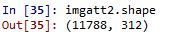
\includegraphics[scale=0.7]{figures/hmm/cod6.jpg}
\caption{Gambar ke-6}
\label{contoh}
\end{figure}
\par
\begin{itemize}
\item Penjelasan : Gambar diatas menampilkan jumlah dari baris dan kolom dari variabel imgatt2.
\par
\par
\end{itemize}
\item Kode Random Forest 7 :
\par
\begin{figure}[ht]
\centering
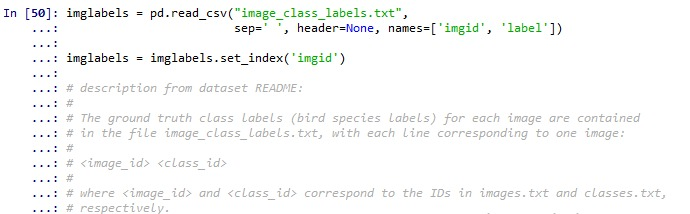
\includegraphics[scale=0.7]{figures/hmm/cod7.jpeg}
\caption{Gambar ke-7}
\label{contoh}
\end{figure}
\par
\begin{itemize}
\item Penjelasan : Gambar di atas menunjukkan hasil muat dari jawabannya yang berisi " apakah burung tersebut ( subjek pada dataset ) termasuk dalam spesies yang mana? Kolom yang digunakan adalah imgid dan label, kemudian melakukan pivot yang mana imgid menjadi index yang artinya unik sehubungan dengan dataset yang telah dieksekusi.
\par
\par
\end{itemize}
\item Kode Random Forest 8 :
\par
\begin{figure}[ht]
\centering
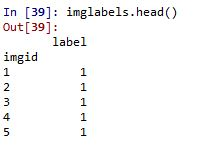
\includegraphics[scale=0.2]{figures/hmm/cod8.jpg}
\caption{Gambar ke-8}
\label{contoh}
\end{figure}
\par
\begin{itemize}
\item Penjelasan : Gambar di atas menunjukkan hasil dari variabel imglabels. Dimana menampilkan dataset dari imgid dan label. Dan dapat dilihat hasilnya dari gambar di atas.
\par
\par
\end{itemize}
\item Kode Random Forest 9 :
\par
\begin{figure}[ht]
\centering
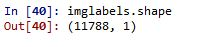
\includegraphics[scale=0.7]{figures/hmm/cod9.jpg}
\caption{Gambar ke-9}
\label{contoh}
\end{figure}
\par
\begin{itemize}
\item Penjelasan : Gambar di atas menunjukkan jumlah baris dan kolom dari variabel imglabels. Dimana hasil dari kodingan tersebut dapat dilihat setelah di run. 
\par
\par
\end{itemize}
\item Kode Random Forest 10 :
\par
\begin{figure}[ht]
\centering
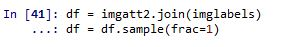
\includegraphics[scale=0.7]{figures/hmm/cod10.jpg}
\caption{Gambar ke-10}
\label{contoh}
\end{figure}
\par
\begin{itemize}
\item Penjelasan : Gambar diatas diakibatkan isi yang sama, maka dapat melakukan join antara dua data yang diesekusi ( yaitu ada imgatt2 dan imglabels ), sehingga pada hasilnya akan didapatkan data ciri dan data jawaban sehingga bisa dikategorikan/dikelompokkan sebagai supervised learning. Jadi perintah untuk menggabungkan kedua data, kemudian dilakukan pemisahan antara data set untuk training dan test pada dataset yang dieksekusi.
\par
\par
\end{itemize}
\item Kode Random Forest 11 :
\par
\begin{figure}[ht]
\centering
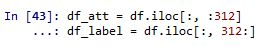
\includegraphics[scale=0.7]{figures/hmm/cod11.jpg}
\caption{Gambar ke-11}
\label{contoh}
\end{figure}
\par
\begin{itemize}
\item Penjelasan : Gambar di atas menghasilkan pemisahan dan pemilihan tabel ( memisahkan dan memilih tabel ). 
\par
\par
\end{itemize}
\item Kode Random Forest 12 :
\par
\begin{figure}[ht]
\centering
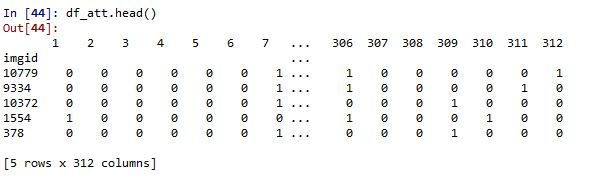
\includegraphics[scale=0.7]{figures/hmm/cod12.jpg}
\caption{Gambar ke-12}
\label{contoh}
\end{figure}
\par
\begin{itemize}
\item Penjelasan : Gambar di atas menunjukkan hasil dari variabel dtatthead yang dimana data nya dapat dilihat pada gambar diatas. Dan dataset nya terdiri dari 5 baris dan 312 kolom.
\par
\par
\end{itemize}
\item Kode Random Forest 13 :
\par
\begin{figure}[ht]
\centering
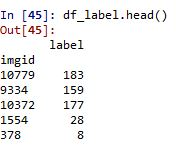
\includegraphics[scale=0.7]{figures/hmm/cod13.jpg}
\caption{Gambar ke-13}
\label{contoh}
\end{figure}
\par
\begin{itemize}
\item Penjelasan : Gambar di atas menunjukkan hasil dari variabel dflabel.head. Dimana berisikan data dari imgid dan label. Dan hasilnya dapat dilihat pada gambar di atas.
\par
\par
\end{itemize}
\item Kode Random Forest 14 :
\par
\begin{figure}[ht]
\centering
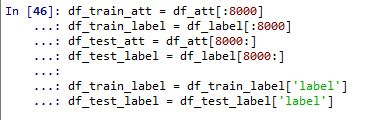
\includegraphics[scale=0.7]{figures/hmm/cod14.jpg}
\caption{Gambar ke-14}
\label{contoh}
\end{figure}
\par
\begin{itemize}
\item Penjelasan : Gambar di atas merupakan pembagian dari data training dan dataset
\par
\par
\end{itemize}
\item Kode Random Forest 15 :
\par
\begin{figure}[ht] 
\centering
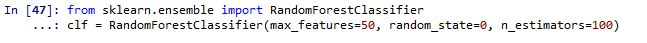
\includegraphics[scale=0.7]{figures/hmm/cod15.jpg}
\caption{Gambar ke-15}
\label{contoh}
\end{figure}
\par
\begin{itemize} 
\item Penjelasan : Gambar di atas merupakan pemanggilan kelas RandomForestClassifier. max features yang diartikan berapa banyak kolom pada setiap tree.
\par
\par
\end{itemize}
\item Kode Random Forest 16 :
\par
\begin{figure}[ht]
\centering
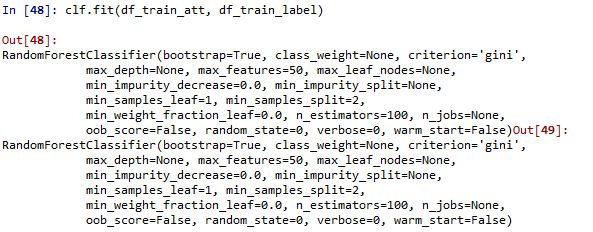
\includegraphics[scale=0.7]{figures/hmm/cod16.jpg}
\caption{Gambar ke-16}
\label{contoh}
\end{figure}
\par
\begin{itemize}
\item Penjelasan : Gambar di atas merupaka perintah untuk melakukan fit untuk membangun random forest yang sudah ditentukan dengan maksimum fitur sebanyak 50.
\par
\par
\end{itemize}
\item Kode Random Forest 17 :
\par
\begin{figure}[ht]
\centering
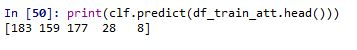
\includegraphics[scale=0.7]{figures/hmm/cod17.jpg}
\caption{Gambar ke-17}
\label{contoh}
\end{figure}
\par
\begin{itemize}
\item Penjelasan : Gambar di atas menunjukkan hasil dari cetakan variabel dftrainatt.head.
\par
\par
\end{itemize}
\item Kode Random Forest 18 :
\par
\begin{figure}[ht]
\centering
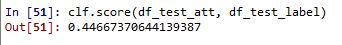
\includegraphics[scale=0.7]{figures/hmm/cod18.jpg}
\caption{Gambar ke-18}
\label{contoh}
\end{figure}
\par
\begin{itemize}
\item Penjelasan : Gambar di atas merupakan hasil dari variabel dftestatt da dftsetlabel. Dimana hasilnya dapat dilihat dari pada gambar di atas
\par
\par
\end{itemize}

\end{itemize}


\par
\par
\item Program Aplikasi Confusion Matrix dan Penjelasan Keluarannya :
\begin{itemize}
\item Kode Confusion Matrix 1 :
\par
\begin{figure}[ht]
\centering
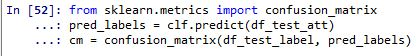
\includegraphics[scale=0.7]{figures/hmm/cod19.jpg}
\caption{Gambar ke-19}
\label{contoh}
\end{figure}
\par
\begin{itemize}
\item Penjelasan :  Gambar di atas merupakan kodingan untuk import confusiion matrik dari random forest. untuk hasilnya dapat dilihat dari gambar.
\par 
\par
\end{itemize}
\item Code Confusion Matrix 2 :
\par
\begin{figure}[ht]
\centering
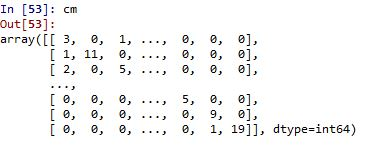
\includegraphics[scale=0.7]{figures/hmm/cod20.jpg}
\caption{Gambar ke-20}
\label{contoh}
\end{figure}
\par
\begin{itemize}
\item Penjelasan : Gambar di atas merupakan tampilan dari variabel cm.
\par
\par
\end{itemize}
\item Kode Confusion Matrix 3 :
\par
\begin{figure}[ht]
\centering
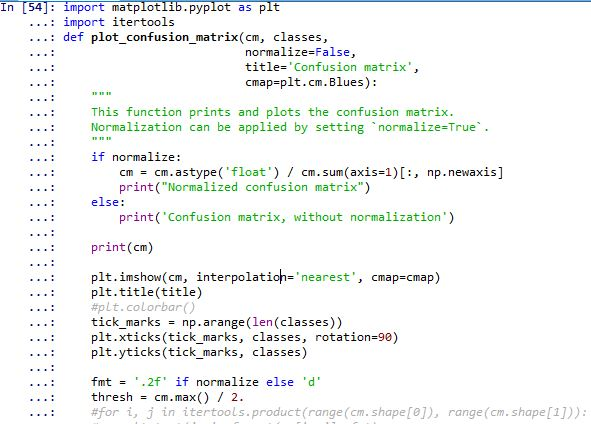
\includegraphics[scale=0.7]{figures/hmm/cod21.jpg}
\caption{Gambar ke-21}
\label{contoh}
\end{figure}
\par
\begin{itemize}
\item Penjelasan : Gambar di atas merupakan perintah untuk plot. Dan untuk hasilnya terpadat pada gambar di atas. 
\par
\par
\end{itemize}
\item Kode Confusion Matrix 4 :
\par
\begin{figure}[ht]
\centering
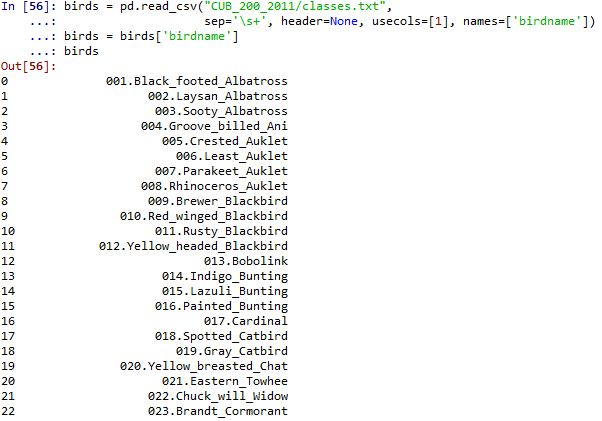
\includegraphics[scale=0.7]{figures/hmm/cod22.jpg}
\caption{Gambar ke-22}
\label{contoh}
\end{figure}
\par
\begin{itemize}
\item Penjelasan : Gambar di atas merupakan kodingan untuk menyesuaikan sumbu dengan nama datanya makanya datset nya di lakukan dengan perintah di atas.
\par
\par
\par
\end{itemize}
\item Kode Confusion Matrix 5 :
\par
\begin{figure}[ht]
\centering
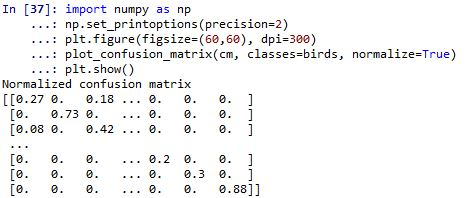
\includegraphics[scale=0.7]{figures/hmm/cod23.jpeg}
\caption{Gambar ke-23}
\label{contoh}
\end{figure}
\par
\begin{itemize}
\item Penjelasan : Gambar di atas merupakan perintah plot dari gambar sebelumnya.
\par
\par
\par
\end{itemize}

\end{itemize}

\par
\par
\item Program Klasifikasi SVM dan Decision Tree Beserta Penjelasan Keluarannya :
\begin{itemize}
\item Kode SVM :
\par
\begin{figure}[ht]
\centering
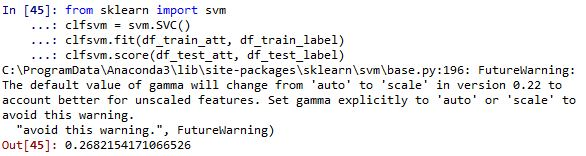
\includegraphics[scale=0.7]{figures/hmm/cod25.jpg}
\caption{Gambar SVM}
\label{contoh}
\end{figure}
\par
\begin{itemize}
\item Penjelasan : Pada gambar di atas cara untuk mencoba klasikasi dengan SVM dengan dataset yang sama.
\par 
\par
\end{itemize}
\item Kode Decision Tree :
\par
\begin{figure}[ht]
\centering
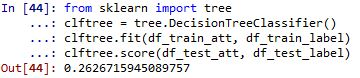
\includegraphics[scale=0.7]{figures/hmm/cod24.jpg}
\caption{Decission Tree}
\label{contoh}
\end{figure}
\par
\begin{itemize}
\item Penjelasan : Pada gambar di atas merupakan cara untuk mencoba klasikasi dengan decission tree dengan dataset yang sama.
\par
\par
\end{itemize}
\end{itemize}



\par
\par
\item Program Cross Validation dan Penjelasan Keluarannya :
\begin{itemize}
\item Code Cross Validation 1 :
\par
\begin{figure}[ht]
\centering
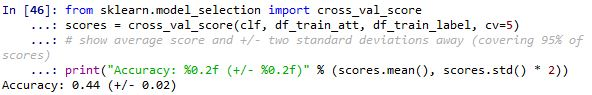
\includegraphics[scale=0.7]{figures/hmm/cod26.jpg}
\caption{Cross Validation 1}
\label{contoh}
\end{figure}
\par
\begin{itemize}
\item Penjelasan : Pada gambar di atas merupakan Hasil dari cross validation random forest.
\par 
\par
\end{itemize}
\item Code Cross Validation 2  :
\par
\begin{figure}[ht]
\centering
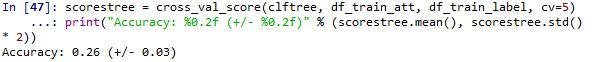
\includegraphics[scale=0.7]{figures/hmm/cod27.jpg}
\caption{Cross Validation 2}
\label{contoh}
\end{figure}
\par
\begin{itemize}
\item Penjelasan : Pada gambar di atas merupakan hasil dari cross validation Decission tree.
\par
\par
\end{itemize}
\item Code Cross Validation 3 :
\par
\begin{figure}[ht]
\centering
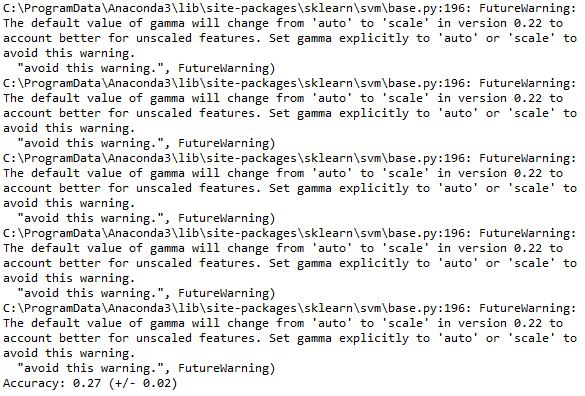
\includegraphics[scale=0.7]{figures/hmm/cod28.jpg}
\caption{Cross Validation 3}
\label{contoh}
\end{figure}
\par
\begin{itemize}
\item Penjelasan : Pada gambar di atas merupakan hasil dari cross validation SVM.
\par
\par
\end{itemize}
\end{itemize}

\par
\par
\item Program Pengamatan Komponen Informasi dan Penjelasan Keluarannya :
\begin{itemize}
\item Code Pengamatan Komponen Informasi 1 :
\par
\begin{figure}[ht]
\centering
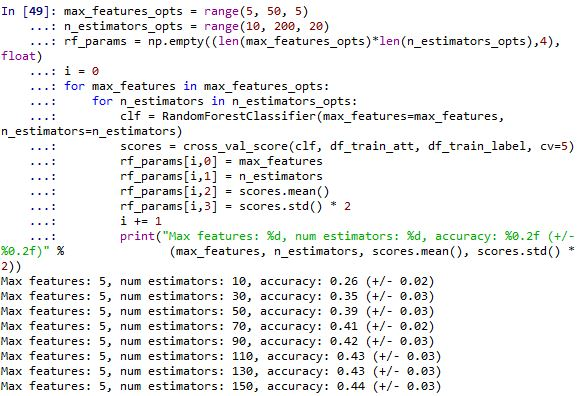
\includegraphics[scale=0.7]{figures/hmm/cod29.jpg}
\caption{Program Pengamatan Komponen Informasi 1}
\label{contoh}
\end{figure}
\par
\begin{itemize}
\item Penjelasan : Pada gambar di atas menunjukkan cara untuk mengetahui berapa banyak tree yang dibuat, berapa banyak atribut yang dipakai dan informasi lainnya menggunakan kode.
\par 
\par
\end{itemize}
\item Code Pengamatan Komponen Informasi 2 :
\par
\begin{figure}[ht]
\centering
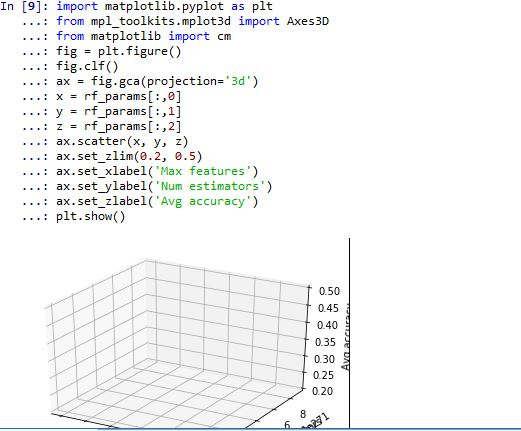
\includegraphics[scale=0.7]{figures/hmm/cod30.jpg}
\caption{Program Pengamatan Komponen Informasi 2}
\label{contoh}
\end{figure}
\par
\begin{itemize}
\item Penjelasan : Pada gambar di atas merupakan cara untuk  melakukan plot informasi ini dengan kode di atas.
\par 
\par
\end{itemize}
\end{itemize}
\end{itemize}
\end{itemize}

\item Penanganan Error
\begin{itemize}
\item Skrinsut Error
\par
\begin{figure}[ht]
\centering
\includegraphics[scale=0.7]{figures/hmm/errorr.jpg}
\caption{Error}
\label{contoh}
\end{figure}
\par
\begin{itemize}
\item Kode Error: file b'data/CUB 200 2011/attributes/image attributes labels.txt'
\par 
\item Solusi Pemecahan Error : Hapus Direktori data pada kode pastikan satu folder.
\par 
\par
\end{itemize}
\end{itemize}

\end{enumerate}

<<<<<<< HEAD

\section {Puad Hamdani / 1164084}
\subsection{Praktek}
Penyelesaian Tugas minggu ke 3
\begin{enumerate}
\item Program Aplikasi Random Forest dan Penjelasan Keluarannya :
\begin{itemize}
\item Code 1 :
\par
\begin{figure}[ht]
\centering
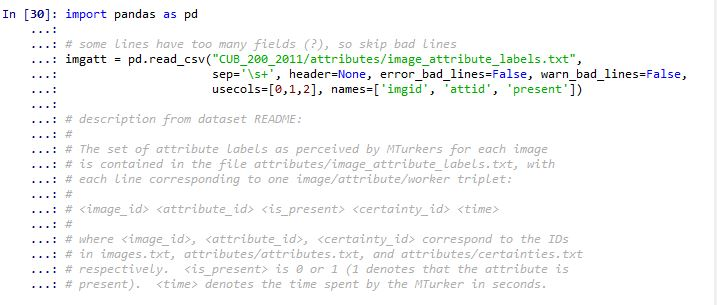
\includegraphics[scale=0.7]{figures/pd1.jpg}
\caption{Gambar1}
\label{contoh}
\end{figure}
\par
\begin{itemize}
\item Penjelasan : Membaca dataset. Codingan di atas menghasilkan variabel baru yaitu imgatt. Terdapat 3 kolom dan 3677856 baris data.
\par 
\par
\end{itemize}
\item Code 2 :
\par
\begin{figure}[ht]
\centering
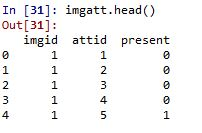
\includegraphics[scale=0.7]{figures/pd2.jpg}
\caption{Gambar2}
\label{contoh}
\end{figure}
\par
\begin{itemize}
\item Penjelasan : Codingan di atas berfungsi untuk melihat sebagian data awal dari dataset. Hasilnya terdapat pada gambar di atas setelah di eksekusi.
\par
\par
\end{itemize}
\item Code  3 :
\par
\begin{figure}[ht]
\centering
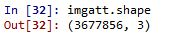
\includegraphics[scale=0.7]{figures/pd3.jpg}
\caption{Gambar3}
\label{contoh}
\end{figure}
\par
\begin{itemize}
\item Penjelasan : Codingan di atas merupakan tampilan untuk menampilkan hasil dari dataset yang telah di run atau di eksekusi. Dimana pada gambar di atas 3677856 merupakan baris dan 3 adalah kolom.
\par
\par
\end{itemize}
\item Code 4 :
\par
\begin{figure}[ht]
\centering
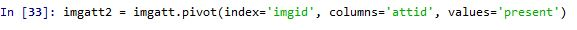
\includegraphics[scale=0.7]{figures/pd4.jpg}
\caption{Gambar 4}
\label{contoh}
\end{figure}
\par
\begin{itemize}
\item Penjelasan : Pada gambar di atas menmapilkan hasil dari variabel imgatt2. Dimana index nya 'imgid', kolom berisi 'attid' dan values atau nilainya berisi 'present'.
\par
\par
\end{itemize}
\item Code 5 :
\par
\begin{figure}[ht]
\centering
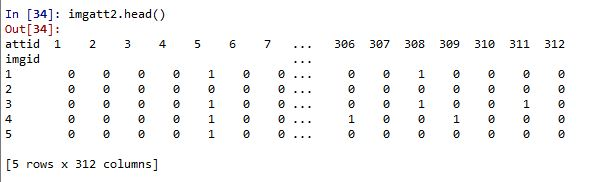
\includegraphics[scale=0.7]{figures/pd5.jpg}
\caption{Gambar 5}
\label{contoh}
\end{figure}
\par
\begin{itemize}
\item Penjelasan : Pada gambar di atas menmapilkan hasil dari variabel imgatt2.head. Dimana dataset nya ada 5 baris dan 312 kolom.
\par
\par
\end{itemize}
\item Code 6 :
\par
\begin{figure}[ht]
\centering
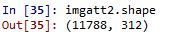
\includegraphics[scale=0.7]{figures/pd6.jpg}
\caption{Gambar 6}
\label{contoh}
\end{figure}
\par
\begin{itemize}
\item Penjelasan : Pada gambar di atas menampilkan jumlah dari baris dan kolom dari variabel imgatt2. Dimana 11788 adalah baris dan 312 adalah kolom.
\par
\par
\end{itemize}
\item Code 7 :
\par
\begin{figure}[ht]
\centering
\includegraphics[scale=0.7]{figures/pd7.jpeg}
\caption{Gambar 7}
\label{contoh}
\end{figure}
\par
\begin{itemize}
\item Penjelasan : Pada gambar di atas menunjukkan load dari  jawabannya yang berisi " apakah burung tersebut ( subjek pada dataset ) termasuk dalam spesies yang mana ?. Kolom yang digunakan adalah imgid dan label, kemudian melakukan pivot yang mana imgid menjadi index yang artinya unik sehubungan dengan dataset yang telah dieksekusi.
\par
\par
\end{itemize}
\item Code 8 :
\par
\begin{figure}[ht]
\centering
\includegraphics[scale=0.2]{figures/pd8.jpg}
\caption{Gambar 8}
\label{contoh}
\end{figure}
\par
\begin{itemize}
\item Penjelasan : Pada gambar di atas menunjukkan hasil dari variabel imglabels. Dimana menampilkan dataset dari imgid dan label. Dan dapat dilihat hasilnya dari gambar di atas.
\par
\par
\end{itemize}
\item Code 9 :
\par
\begin{figure}[ht]
\centering
\includegraphics[scale=0.7]{figures/pd9.jpg}
\caption{Gambar 9}
\label{contoh}
\end{figure}
\par
\begin{itemize}
\item Penjelasan : Pada gambar di atas menunjukkan jumlah baris dan kolom dari variabel imglabels. Dimana hasil dari kodingan tersebut dapat dilihat setelah di run. 
\par
\par
\end{itemize}
\item Code 10 :
\par
\begin{figure}[ht]
\centering
\includegraphics[scale=0.7]{figures/pd10.jpg}
\caption{Gambar 10}
\label{contoh}
\end{figure}
\par
\begin{itemize}
\item Penjelasan : Pada gambar diatas dikarenakan isinya sama, maka bisa melakukan join antara dua data yang diesekusi ( yaitu ada imgatt2 dan imglabels ), sehingga pada hasilnya akan didapatkan data ciri dan data jawaban atau labelnya sehingga bisa dikategorikan/dikelompokkan sebagai supervised learning. Jadi perintah untuk menggabungkan kedua data, kemudian dilakukan pemisahan antara data set untuk training dan test pada dataset yang dieksekusi.
\par
\par
\end{itemize}
\item Code 11 :
\par
\begin{figure}[ht]
\centering
\includegraphics[scale=0.7]{figures/pd11.jpg}
\caption{Gambar 11}
\label{contoh}
\end{figure}
\par
\begin{itemize}
\item Penjelasan :Pada gambar di atas menghasilkan pemisahan dan pemilihan tabel ( memisahkan dan memilih tabel ). 
\par
\par
\end{itemize}
\item Code 12 :
\par
\begin{figure}[ht]
\centering
\includegraphics[scale=0.7]{figures/pd12.jpg}
\caption{Gambar 12}
\label{contoh}
\end{figure}
\par
\begin{itemize}
\item Penjelasan : Pada gambar di atas menunjukkan hasil dari variabel dtatthead. Dimana data nya dapat dilihat pada gambar diatas. Dan dataset nya terdiri dari 5 baris dan 312 kolom.
\par
\par
\end{itemize}
\item Code 13 :
\par
\begin{figure}[ht]
\centering
\includegraphics[scale=0.7]{figures/pd13.jpg}
\caption{Gambar 13}
\label{contoh}
\end{figure}
\par
\begin{itemize}
\item Penjelasan : Pada gambar di atas menunjukkan hasil dari variabel dflabel.head. Dimana berisikan data dari imgid dan label. Dan hasilnya dapat dilihat pada gambar di atas.
\par
\par
\end{itemize}
\item Code 14 :
\par
\begin{figure}[ht]
\centering
\includegraphics[scale=0.7]{figures/pd14.jpg}
\caption{Gambar 14}
\label{contoh}
\end{figure}
\par
\begin{itemize}
\item Penjelasan : Pada gambar di atas merupakan pembagian dari data training dan dataset
\par
\par
\end{itemize}
\item Code 15 :
\par
\begin{figure}[ht] 
\centering
\includegraphics[scale=0.7]{figures/pd15.jpg}
\caption{Gambar 15}
\label{contoh}
\end{figure}
\par
\begin{itemize} 
\item Penjelasan : Pada gambar di atas merupakan pemanggilan kelas RandomForestClassifier. max features yang diartikan berapa banyak kolom pada setiap tree.
\par
\par
\end{itemize}
\item Code 16 :
\par
\begin{figure}[ht]
\centering
\includegraphics[scale=0.7]{figures/pd16.jpg}
\caption{Gambar 16}
\label{contoh}
\end{figure}
\par
\begin{itemize}
\item Penjelasan : Pada gambar di atas merupaka perintah untuk melakukan fit untuk membangun random forest yang sudah ditentukan dengan maksimum fitur sebanyak 50.
\par
\par
\end{itemize}
\item Code 17 :
\par
\begin{figure}[ht]
\centering
\includegraphics[scale=0.7]{figures/pd18.jpg}
\caption{Gambar 17}
\label{contoh}
\end{figure}
\par
\begin{itemize}
\item Penjelasan : Pada gambar di atas menunjukkan hasil dari cetakan variabel dftrainatt.head.
\par
\par
\end{itemize}
\item Code  18 :
\par
\begin{figure}[ht]
\centering
\includegraphics[scale=0.7]{figures/pd18.jpg}
\caption{Gambar 18}
\label{contoh}
\end{figure}
\par
\begin{itemize}
\item Penjelasan : Pada gambar di atas merupakan hasil dari variabel dftestatt da dftsetlabel. Dimana hasilnya dapat dilihat dari pada gambar di atas
\par
\par
\end{itemize}

\end{itemize}


\par
\par
\item Program Aplikasi Confusion Matrix dan Penjelasan Keluarannya :
\begin{itemize}
\item Code 1 :
\par
\begin{figure}[ht]
\centering
\includegraphics[scale=0.7]{figures/pd19.jpg}
\caption{Gambar 19}
\label{contoh}
\end{figure}
\par
\begin{itemize}
\item Penjelasan :  Pada gambar di atas merupakan kodingan untuk import confusiion matrik dari random forest. untuk hasilnya dapat dilihat dari gambar.
\par 
\par
\end{itemize}
\item Code  2 :
\par
\begin{figure}[ht]
\centering
\includegraphics[scale=0.7]{figures/pd20.jpg}
\caption{Gambar 20}
\label{contoh}
\end{figure}
\par
\begin{itemize}
\item Penjelasan : Pada gambar di atas merupakan tampilan dari variabel cm.
\par
\par
\end{itemize}
\item Code  3 :
\par
\begin{figure}[ht]
\centering
\includegraphics[scale=0.7]{figures/pd21.jpg}
\caption{Gambar 21}
\label{contoh}
\end{figure}
\par
\begin{itemize}
\item Penjelasan : Pada gambar di atas merupakan perintah untuk plot. Dan untuk hasilnya terpadat pada gambar di atas. 
\par
\par
\end{itemize}
\item Code  4 :
\par
\begin{figure}[ht]
\centering
\includegraphics[scale=0.7]{figures/pd22.jpg}
\caption{Gambar 22}
\label{contoh}
\end{figure}
\par
\begin{itemize}
\item Penjelasan : Pada gambar di atas merupakan kodingan untuk menyesuaikan sumbu dengan nama datanya makanya datset nya di lakukan dengan perintah di atas.
\par
\par
\par
\end{itemize}
\item Code 5 :
\par
\begin{figure}[ht]
\centering
\includegraphics[scale=0.7]{figures/pd23.jpeg}
\caption{Gambar 23}
\label{contoh}
\end{figure}
\par
\begin{itemize}
\item Penjelasan : Pada gambar di atas merupakan perintah plot dari gambar sebelumnya.
\par
\par
\par
\end{itemize}

\end{itemize}

\par
\par
\item Program Klasifikasi SVM dan Decision Tree Beserta Penjelasan Keluarannya :
\begin{itemize}
\item Code SVM :
\par
\begin{figure}[ht]
\centering
\includegraphics[scale=0.7]{figures/pd24.jpg}
\caption{SVM}
\label{contoh}
\end{figure}
\par
\begin{itemize}
\item Penjelasan : Pada gambar di atas cara untuk mencoba klasikasi dengan SVM dengan dataset yang sama.
\par 
\par
\end{itemize}
\item Code Decision Tree :
\par
\begin{figure}[ht]
\centering
\includegraphics[scale=0.7]{figures/pd25.jpg}
\caption{Decission Tree}
\label{contoh}
\end{figure}
\par
\begin{itemize}
\item Penjelasan : Pada gambar di atas merupakan cara untuk mencoba klasikasi dengan decission tree dengan dataset yang sama.
\par
\par
\end{itemize}
\end{itemize}



\par
\par
\item Program Cross Validation dan Penjelasan Keluarannya :
\begin{itemize}
\item Code 1 :
\par
\begin{figure}[ht]
\centering
\includegraphics[scale=0.7]{figures/pd26.jpg}
\caption{Cross Validation 1}
\label{contoh}
\end{figure}
\par
\begin{itemize}
\item Penjelasan : Pada gambar di atas merupakan Hasil dari cross validation random forest.
\par 
\par
\end{itemize}
\item Code  2  :
\par
\begin{figure}[ht]
\centering
\includegraphics[scale=0.7]{figures/pd27.jpg}
\caption{Cross Validation 2}
\label{contoh}
\end{figure}
\par
\begin{itemize}
\item Penjelasan : Pada gambar di atas merupakan hasil dari cross validation Decission tree.
\par
\par
\end{itemize}
\item Code  3 :
\par
\begin{figure}[ht]
\centering
\includegraphics[scale=0.7]{figures/pd28.jpg}
\caption{Cross Validation 3}
\label{contoh}
\end{figure}
\par
\begin{itemize}
\item Penjelasan : Pada gambar di atas merupakan hasil dari cross validation SVM.
\par
\par
\end{itemize}
\end{itemize}
\par
\par
\item Program Pengamatan Komponen Informasi dan Penjelasan Keluarannya :
\begin{itemize}
\item Code 1 :
\par
\begin{figure}[ht]
\centering
\includegraphics[scale=0.7]{figures/pd29.jpg}
\caption{Program Pengamatan Komponen Informasi 1}
\label{contoh}
\end{figure}
\end{itemize}
\par
\begin{itemize}
\item Penjelasan : Pada gambar di atas menunjukkan cara untuk mengetahui berapa banyak tree yang dibuat, berapa banyak atribut yang dipakai dan informasi lainnya menggunakan kode.
\par 
\par


\item Code 2 :
\par
\begin{figure}[ht]
\centering
\includegraphics[scale=0.7]{figures/pd30.jpg}
\caption{Program Pengamatan Komponen Informasi 2}
\label{contoh}
\end{figure}
\end{itemize}
\par
\begin{itemize}
\item Penjelasan : Pada gambar di atas merupakan cara untuk  melakukan plot informasi ini dengan kode di atas.
\par 
\par
\end{itemize}


\item Penanganan Error
\begin{itemize}
\item Skrinsut Error
\par
\begin{figure}[ht]
\centering
\includegraphics[scale=0.7]{figures/Error.jpg}
\caption{Error}
\label{contoh}
\end{figure}
\end{itemize}
\par
\begin{itemize}
\item Kode Error: file b'data/CUB 200 2011/attributes/image attributes labels.txt'
\par 
\item Solusi Pemecahan Error : Hapus Direktori data pada kode pastikan satu folder.
\par 
\par
\end{itemize}
\end{enumerate}

=======
\section {Mhd Zulfikar Akram Nasution / 1164081}
\subsection {Teori}
\begin{enumerate}
\item Random Forest
\par
Ramdom Forest adalah hutan yang acak, dimana maksudnya yaitu terdapat banyak pohon-pohon yang mana disetiap pohon tersebut memiliki atribut yang berbeda-beda, random forest disebut juga kumpulan pohon-pohon keputusan. contoh random forest seperti gambar 3.1
\begin{figure}[ht]
\centering
\includegraphics[scale=0.6]{figures/RF/1_1.png}
\caption{Random Forest}
\end{figure}
\item Cara membaca dataset kasus
\item Buka aplikasi spyder untuk membuka dan membaca kodingan dataset
\item Kemudian buat  variable imgatt untuk memasukkan atribut label
\item Lalu uji coba kodingan untuk mengetahui apa hasil dari dataset tersebut
\item imgatt.head() untuk melihat sebagian data awal
\item .shape untuk melihat jumlah data
\item .pivot untuk merubah atribut menjadi kolom
\par
Dengan menguji coba kodingan yang ada pada spyder kita akan dapat membaca dataset yang ada.
\item Cross Validation
\par 
Cross Validation adalah sebuah metode statistik yang digunakan untuk mengevaluasi kinerja model, dimana data dipisah menjadi dua subset yaitu data proses pembelajan dan data evaluasi atau validasi.
\item Arti 44 persen pada RF, 27 persen pada Decission Tree, dan 29 persen pada SVM.
\item 44 persen pada Random Forest adalah menjunjukkan hasil yang sempurna pada keputusan yang diambil, biasanya hasil keputusan yang dicapai sekitar 42-44 persen.
\item 27 persen pada Decission Tree adalah menunjukkan hasil keputusan pada tiap-tiap tree dari dataset yang ada.
\item 29 persen pada SVM menunjukkan hasil keputusan dengan klasifikasi dari dataset yang ada.
\item Confusion Matrix
\item Pertama import confusion matrixnya
\item Kemudian Plot confusion matrix
\item Lalu sesuaikan plotnya dengan nama data yang ada
\item Setelah itu plot kembali
\par
Contoh hasil connfusion matrix pada gambar 3.2
\begin{figure}[ht]
\centering
\includegraphics[scale=0.9]{figures/RF/1_2.png}
\caption{Confusion Matrix}
\end{figure}
\item Voting
\par
Voting adalah hasil akhir dari keputusan yang ada pasa setiap pohon di random forest, maksudnya ialah setiap keputusan yang telah dikumpulkan maka akan di voting bahwa hasil tersebut adalah hasil yang benar. Misalnya kita dapat lihat pada gambar 3.3 yaitu dari beberapa ciri-ciri yang ada dapat di voting atau disimpilkan hasil yang paling banyak dimiliki oleh burung belibis, sehingga dapat disimpulkan bahwa dari ciri- tersebut ialah merupakan ciri-ciri dari burung belibis. 
\begin{figure}[ht]
\centering
\includegraphics[scale=0.9]{figures/RF/1_2.png}
\caption{Voting}
\end{figure}
\end{enumerate}
\subsection{Praktek}
\begin{enumerate}
\item Aplikasi sederhana menggunakan Pandas seperti pada gambar 3.14
	\begin{figure}[ht]
	\centering
	\includegraphics[scale=0.7]{figures/PRF/1_1.png}
	\caption{Aplikasi pandas}
	\end{figure}
	\par Penjelasan kodingan :
		\begin{itemize}
		\item Memanggil library.
		\item Membuat variable dengan data frame.
		\item Menampilkan hasil
		\end{itemize}
	\par Sehingga menghasilkan gambar 3.15 :
	\begin{figure}[ht]
	\centering
	\includegraphics[scale=0.7]{figures/PRF/1_2.png}
	\caption{Hasil Pandas}
	\end{figure}
\item Aplikasi sederhana menggunakan Numpy pada gambar 3.16
	\begin{figure}[ht]
	\centering
	\includegraphics[scale=0.9]{figures/PRF/2_1.png}
	\caption{Aplikasi Numpy}
	\end{figure}
	\par Penjelasan kodingan :
		\begin{itemize}
		\item Memanggil library
		\item Membuat variable dengan value random dan size 3
		\item Menampilkan hasil value
		\end{itemize}
	\par Sehingga menghasilkan gambar 3.17:
	\begin{figure}[ht]
	\centering
	\includegraphics[scale=0.9]{figures/PRF/2_1.png}
	\caption{Hasil Numpy}
	\end{figure}
\item Aplikasi sederhana menggunakan Matplotlib pada gambar 3.18
	\begin{figure}[ht]
	\centering
	\includegraphics[scale=0.7]{figures/PRF/3_1.png}
	\caption{Aplikasi Matplotlib}
	\end{figure}
	\par Penjelasan kodingan :
		\begin{itemize}
		\item Memanggil library
		\item Membuat variable yang berisi bahasa pemrograman
		\item Membuat variable yang berisi popularitas
		\item Membuat variable untuk explode
		\item Membuat diagram pie atau yang berbentuk lingkaran
		\item Membuat garis koordinat
		\item Menampilkan hasil
		\end{itemize}
	\par Sehingga menghasilkan gambar 3.19:
	\begin{figure}[ht]
	\centering
	\includegraphics[scale=0.7]{figures/PRF/3_2.png}
	\caption{Hasil Matplotlib}
	\label{contoh}
	\end{figure}
\item Program klasifikasi random forest
	\begin{itemize}
		\item Pertama baca dataset terlebih dahulu seperti pada gambar 3.20
			\begin{figure}[ht]
			\centering
			\includegraphics[scale=0.7]{figures/PRF/4_1.png}
			\caption{Membaca Data File}
			\end{figure}
		\item Kemudian lihat sebagian data awal dengan listing seperti pada gambar 3.21
			\begin{figure}[ht]
			\centering
			\includegraphics[scale=0.9]{figures/PRF/4_2.png}
			\caption{Melihat sebagian data}
			\end{figure}
		\item Kemudian lihat jumlah datal dengan listing seperti pada gambar 3.22
			\begin{figure}[ht]
			\centering
			\includegraphics[scale=0.9]{figures/PRF/4_3.png}
			\caption{Melihat jumlah data}
			\end{figure}
		\item Ubah atribut menjadi kolom seperti pada gambar 3.23
			\begin{figure}[ht]
			\centering
			\includegraphics[scale=0.7]{figures/PRF/4_4.png}
			\caption{Ubah atribut jadi kolom}
			\end{figure}
		\item Membaca dataset label seperti pada gambar 3.24
			\begin{figure}[ht]
			\centering
			\includegraphics[scale=0.7]{figures/PRF/4_5.png}
			\caption{Membaca dataset label}
			\end{figure}
		\item Menggabungkan field dari dua file terpisah seperti pada gambar 3.25
			\begin{figure}[ht]
			\centering
			\includegraphics[scale=0.9]{figures/PRF/4_6.png}
			\caption{Menggabungkan field}
			\end{figure}
		\item Memidahkan dan memilih label seperti pada gambar 3.26
			\begin{figure}[ht]
			\centering
			\includegraphics[scale=0.9]{figures/PRF/4_7.png}
			\caption{Memisahkan dan memilih label}
			\end{figure}
		\item Melihat isi masing-masing data frame seperti pada gambar 3.27
			\begin{figure}[ht]
			\centering
			\includegraphics[scale=0.9]{figures/PRF/4_8.png}
			\caption{Melihat isi data}
			\end{figure}
		\item Pembagian data training dan data tes seperti pada gambar 3.28
			\begin{figure}[ht]
			\centering
			\includegraphics[scale=0.9]{figures/PRF/4_9.png}
			\caption{Pembagian data}
			\end{figure}
		\item Memanggil kelas random forest seperti pada gambar 3.29
			\begin{figure}[ht]
			\centering
			\includegraphics[scale=0.7]{figures/PRF/4_10.png}
			\caption{Kelas random forest}
			\end{figure}
		\item Lakukan fit untuk emmbangun random forest seperti pada gambar 3.30
			\begin{figure}[ht]
			\centering
			\includegraphics[scale=0.7]{figures/PRF/4_11.png}
			\caption{Membuat fitting}
			\end{figure}
		\item Kemudian lihat hasil dengan predict seperti pada gambar 3.31
			\begin{figure}[ht]
			\centering
			\includegraphics[scale=0.9]{figures/PRF/4_12.png}
			\caption{Melihat hasil}
			\end{figure}
		\item Lalu akan terlihat hasil score dari klasifikasi seperti pada gambar 3.32
			\begin{figure}[ht]
			\centering
			\includegraphics[scale=0.9]{figures/PRF/4_13.png}
			\caption{Hasil score}
			\end{figure}
	\end{itemize}
\item Program Klasifikasi Confusion Matrix
	\begin{itemize}
		\item Setelah melakukan random forest kemudian dipetakan ke dalam confusion matrix seperti pada gambar 3.33
			\begin{figure}[ht]
			\centering
			\includegraphics[scale=0.7]{figures/PRF/5_1.png}
			\caption{Memetakan ke confusion matrix}
			\end{figure}
		\item Kemudian lihat hasilnya seperti pada gambar 3.34
			\begin{figure}[ht]
			\centering
			\includegraphics[scale=0.7]{figures/PRF/5_2.png}
			\caption{Melihat hasil}
			\end{figure}
		\item Lalu lakukan perintah plot seperti pada gambar 3.35
			\begin{figure}[ht]
			\centering
			\includegraphics[scale=0.7]{figures/PRF/5_3.png}
			\caption{Melakukan Plot}
			\end{figure}
		\item Selanjutnya nama data akan di set agar plot sumbunya sesuai seperti pada gambar 3.36
			\begin{figure}[ht]
			\centering
			\includegraphics[scale=0.7]{figures/PRF/5_4.png}
			\caption{Plotting nama data}
			\end{figure}
		\item Setelah label berubah, maka dilakukan perintah plot seperti pada gambar 3.37
		\begin{figure}[ht]
			\centering
			\includegraphics[scale=0.7]{figures/PRF/5_5.png}
			\caption{Melakukan perintah plot}
			\end{figure}
	\end{itemize}
\item Program Klasifikasi SVM dan Decision Tree
	\begin{itemize}
		\item Program Decision Tree seperti pada gambar 3.38
			\par Mengklasifikasikan dataset yang sama menggunakan decision tree.
				\begin{figure}[ht]
				\centering
				\includegraphics[scale=0.7]{figures/PRF/6_1.png}
				\caption{Klasifkasi menggunakan decision tree}
				\end{figure}
		\item Program Klasifikasi SVM seperti pada gambar 3.39
			\par Mengklasifikasikan dataset yang sama menggunakan SVM.
				\begin{figure}[ht]
				\centering
				\includegraphics[scale=0.7]{figures/PRF/6_2.png}
				\caption{Klasifikasi menggunakan SVM}
				\end{figure}
	\end{itemize}
\item Program Cross Validation
	\begin{itemize}
		\item Lakukan pengecekan cross validation untuk random forest seperti pada gambar 3.40
			\begin{figure}[ht]
			\centering
			\includegraphics[scale=0.7]{figures/PRF/7_1.png}
			\caption{Pengecekan cross validation random forest}
			\end{figure}
		\item  Lakukan pengecekan cross validation untuk decission tree  seperti pada gambar 3.41
			\begin{figure}[ht]
			\centering
			\includegraphics[scale=0.7]{figures/PRF/7_2.png}
			\caption{Pengecekan cross validation decision tree}
			\end{figure}
		\item Lakukan pengecekan cross validation untuk SVM  seperti 2pada gambar 3.4
			\begin{figure}[ht]
			\centering
			\includegraphics[scale=0.7]{figures/PRF/7_3.png}
			\caption{Pengecekan cross validation SVM}
			\end{figure}
	\end{itemize}
\item Program Pengamatan Komponen Informasi
	\begin{itemize}
		\item Melakukan pengamatan komponen informasi untuk menetahui berapa banyak tree yang dibuat, atribut yang dipakai, dan informasi lainnya  seperti pada gambar 3.43
			\begin{figure}[ht]
			\centering
			\includegraphics[scale=0.7]{figures/PRF/8_1.png}
			\caption{Pengamatan Komponen}
			\end{figure}
		\item Melakukan plot informasi agar bisa dibaca  seperti pada gambar 3.44
			\begin{figure}[ht]
			\centering
			\includegraphics[scale=0.7]{figures/PRF/8_2.png}
			\caption{Plot informasi}
			\end{figure}
	\end{itemize}
\end{enumerate}





>>>>>>> c781ac4472a25ed2af92e92a48bac83484ece61c
\section{Method 1}
Definition, steps, algoritm or equation of method 1 and how to apply into your data
\section{Method 2}
Definition, steps, algoritm or equation of method 2 and how to apply into your data